% The first argument is the \documentclass, which tells latex which template
% we're using to build this document. It's usually safe to just use "article".
\documentclass{article}

% include some packages...
\usepackage{fullpage} % change settings for a smaller margin
\usepackage{graphicx} % gives access to the \includegraphics commands
\usepackage{amsfonts}
\usepackage{float}
\usepackage{enumitem}
\graphicspath{{./images/}}

% tell Latex to use no paragraph indentation, but leave some space between
% paragraphs 
\setlength{\parindent}{0in}
\setlength{\parskip}{0.1in}

\newcommand{\tib}[1]{\textit{\textbf{#1}}}
\newcommand{\code}[1]{\texttt{#1}}

% these commands merely set the values for the title/date/author; they don't put
% them in the document... see \maketitle below
\title{CS Department Automated Information Timeline. \\ Assignment 2.1: Use Case, Use Case Diagram, System Sequence Diagram, and System Operations}
\date{\today}
\author{Matthew Hays, Pawan Bhandari, Sarah Faron, Tim Klimpel}

% all document content goes between \begin{document} and \end{document}
\begin{document}

% this command actually creates the title/date/author in the document
\maketitle
\newpage
\tableofcontents
\listoffigures
\newpage

\section{Requirements}
\subsection{Functional Requirements}
\begin{enumerate}
    \item \textbf{REQ01}: Faculty members can create a post for review, which will initially default to a proposed state until approved.
    \item \textbf{REQ02}: An admin/reviewer must approve a post before it can be published to the site.
    \item \textbf{REQ03}: A user can add events to an event calendar that can be displayed on screen.
    \item \textbf{REQ04}: A user can add pictures to posts.
    \item \textbf{REQ05}: A user can add videos to posts.
    \item \textbf{REQ06}: A user can add HTML pages to posts.
    \item \textbf{REQ07}: Created posts that will be displayed on a large format screen.
    \item \textbf{REQ08}: The system will allow management of which posts are displayed.
    \item \textbf{REQ09}: The system will allow management of which media is displayed.
    \item \textbf{REQ10}: The system will fall back to the 10 most recent posts if no posts are tagged, or less than 10 posts are tagged.
    \item \textbf{REQ11}: The Office manager will use the WYSIWYG editor to modify static content posts. 
    \item \textbf{REQ12}: The Office Manager will use the WYSIWYG editor to tag posts for display on screen.
    \item \textbf{REQ13}: The system will allow audiences to use their mobile devices (e.g., through a QR code that brings them to the website) to browse all content beyond the 10 most recent posts.
    \item \textbf{REQ14}: The system will allow audiences to use their mobile device to browse the calendar.
    \item \textbf{REQ15}: A user will authenticate and be assigned a valid role or view the content as a non-authenticated user.
\end{enumerate}
\subsection{Non Functional Requirements}
\begin{enumerate}
    \item \textbf{REQ16}: The system will have the following user roles: Faculty, Admin, and Office Manager.
    \item \textbf{REQ17}: Content rolling and updates to content will be completed via WebSockets.
    \item \textbf{REQ18}: The backend will consist of a Spring Framework REST API with a database and appropriate middleware.
    \item \textbf{REQ19}:  The system will manage a media library which consists of all posted pictures and videos.
    \item \textbf{REQ20}: The system will consist of a front-end display: a television screen.
    \item \textbf{REQ21}: The system will consist of a front-end display: a web-based display optimized for all screen sizes.
    \item \textbf{REQ22}:  The design of the user interface must utilize Baylor’s official color scheme:
    \item \textbf{REQ23}: The system will have a WYSIWYG editor.
\end{enumerate}
\subsection{Requirement Priorities}

\begin{table}[H]
    \centering
    \begin{tabular}{| c | c | c | c |}
    \hline
        \textbf{Critical} & \textbf{High} & \textbf{Medium} & \textbf{Low}\\
        \hline
         REQ01 & REQ08 & REQ13 & REQ04 \\
         REQ02 & REQ09 & REQ14 & REQ05 \\
         REQ03 & REQ10 & REQ21 & REQ06 \\
         REQ07 & REQ11 & REQ23 & REQ22 \\
         REQ15 & REQ12 &  & \\
         REQ16 & REQ17 &  & \\
         REQ18 & REQ20 &  & \\
         REQ19 &  &  & \\
    \hline
    \end{tabular}
    \caption{Requirement priorities}
    \label{tab:my_label}
\end{table}
\section{Use Case diagrams}
\begin{figure}[H]
    \centering
    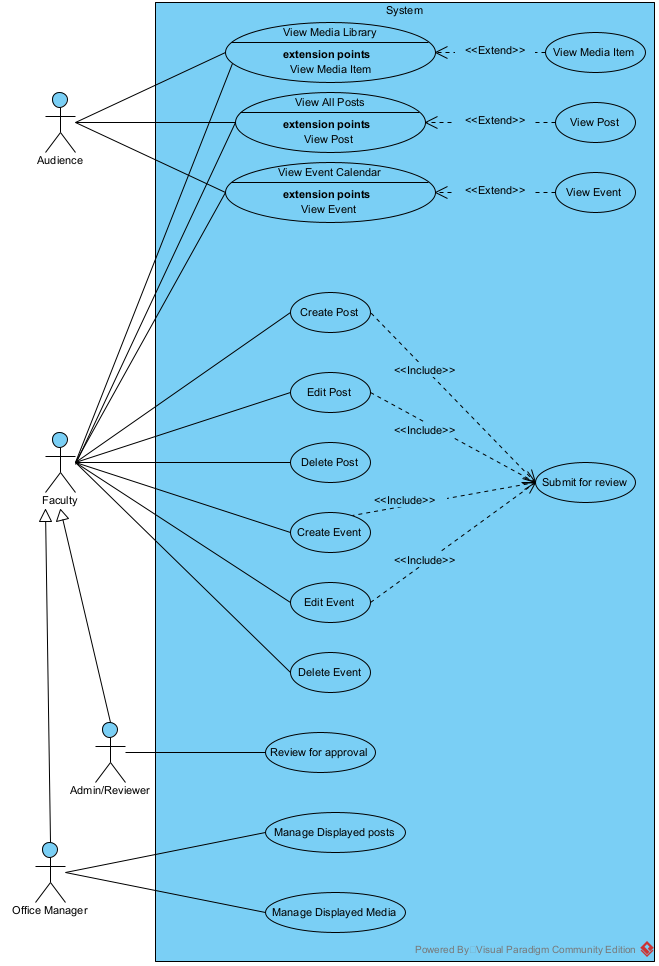
\includegraphics[scale=0.8]{images/UCD.png}
    \caption{Use Case Diagram}
    \label{fig:enter-label}
\end{figure}
\section{Fully dressed use cases}
\subsection{\textbf{UC04}: Create Event (Matthew Hays)}
\textbf{Scope}: CS Automated Information Timeline\\
\\
    \textbf{Level}: User Goal\\
    \\
    \textbf{Stakeholders and Interests}:
    \begin{itemize}[label={}]
         \item \textbf{Faculty}: A person that works for the university and is interested in gaining visibility of their post and/or event.
          \item \textbf{Admin/Reviewer}: A person that works for the university and approves and/or removes posts and/or events from the system. 
    \end{itemize}
    \textbf{Preconditions}:
    \begin{itemize}[label={}]
        \item Faculty has been identified and authenticated.
    \end{itemize}
    \textbf{Postconditions}:
        \begin{itemize}[label={}]
        \item Event has been persisted.
        \item Event has been placed in the proposed state.
        \item An event notification has been persisted.
    \end{itemize}
    \textbf{Main Success Scenario}:
    \begin{enumerate}
        \item Faculty writes the event using the event creation tool.
        \begin{enumerate}
            \item The event title is written by the faculty user.
            \item The event body is written by the faculty user.
        \end{enumerate}
        \item Faculty reviews the event draft.
        \item Faculty submits the event to the system.
        \begin{enumerate}
            \item An event id is generated by the system. 
            \item A timestamp is generated by the system.
            \item The user id of the faculty user is attached to the event object.
            \item The system assigns the status of the event to the proposed state. 
        \end{enumerate}
        \item The system generates a notification object.
        \begin{enumerate}
            \item The event object is attached to the notification object.
        \end{enumerate}
        \item The notification object is persisted.
        \item The event object is persisted.
        \item The system returns the persisted event object to the faculty user.
    \end{enumerate}
    \textbf{Extensions:}
    \begin{enumerate}
        \item[*.a.] Anytime the system does not respond,
        \begin{enumerate}
            \item[1.] Faculty will notify the Admin/Reviewer.
            \item[2.] Admin/Reviewer will restart the system.
        \end{enumerate}
        \item [1.a.]  If the event creation tool does not function,
        \begin{enumerate}
            \item[1.] Faculty reloads the page.
        \end{enumerate}
        \item [5.a.] If the notification is not persisted,
        \begin{enumerate}
            \item [1.] The system returns an error message to the faculty user. 
            \item[2.] The faculty user resubmits the event. 
        \end{enumerate}
        \item [6.a.] If the event is not persisted,
        \begin{enumerate}
            \item [1.] The system returns an error message to the faculty user. 
            \item [2.] Faculty reattempts the submission of the event.
        \end{enumerate}
    \end{enumerate}   
\subsection{\textbf{UC05}: Edit Event (Sarah Faron)}
\textbf{Scope}: CS Automated Information Timeline\\
\\
    \textbf{Level}: User Goal\\
    \\
    \textbf{Stakeholders and Interests}:
    \begin{itemize}[label={}]
        \item \textbf{Audience}: A person that is interested in viewing all approved content on the system using their mobile device.
         \item \textbf{Faculty}: A person that works for the university and is interested in gaining visibility of their post and/or event.
         \item \textbf{Office Manager}: A person that works for the university and is interested in prioritizing the order of posts and/or events. 
          \item \textbf{Admin/Reviewer}: A person that works for the university and approves and/or removes posts and/or events from the system. 
    \end{itemize}
    \textbf{Preconditions}:
    \begin{itemize}[label={}]
        \item Faculty created an event (UC04) and submitted it for review (UC08).
        \item Admin/Reviewer reviewed the event (UC09) and approved.
        \item Admin/Reviewer is identified and authenticated in the system.
        \item Faculty is identified and authenticated in the system and is viewing the event calendar (UC03).
    \end{itemize}
    \textbf{Postconditions}:
        \begin{itemize}[label={}]
        \item Event status is changed from an approved state to a proposed state. 
    \end{itemize}
    \textbf{Main Success Scenario}:
    \begin{enumerate}
        \item Faculty clicks the “Update existing event” link on the event calendar page.
        \item System returns a list of existing events authored by Faculty that have been approved.
        \item Faculty selects the event they wish to edit from the returned list of their previously approved events.
        \item Faculty enters the updated event information into the submission form:
        \begin{enumerate}
            \item Event date 
            \item Event time 
            \item Event description  
        \end{enumerate}
        \item Faculty submits the updated event information for Admin/Reviewer review.
        \item System provides Faculty with a submission confirmation message.
    \end{enumerate}
    \textbf{Extensions:}
    \begin{enumerate}
        \item[3-4.a.] Faculty begins editing the event, then decides not to submit the updates for review,
        \begin{enumerate}
            \item[1.] Upon leaving the web page, any changes to event date, time, or description entered into the submission form are erased.
            \item[2.] Selected event remains unchanged in the system.
        \end{enumerate}
        \item [3.b.]  Faculty does not see the event they wish to edit in the returned list because the event has not yet been approved by the Admin/Reviewer,
        \begin{enumerate}
            \item[1.] Faculty must wait for approval from Admin/Reviewer on the original event before the event is eligible for editing.
        \end{enumerate}
    \end{enumerate}
    \textbf{Special Requirements:} None\\
    \\
    \textbf{Technology and Data Variations List}:
    \begin{enumerate}
        \item[4.a] Date input is required in the format MM/DD/YYYY. 
        \item[4.b] Time input is required in the Standard Time format in the Central Time Zone.
    \end{enumerate}
    \textbf{Frequency of Occurrence}:\\
    Could be nearly continuous if Admin/Reviewer also reviews edited events and approves them (UC09) nearly continuously.\\
    \\
    \textbf{Open Issues}: None
    
\subsection{\textbf{UC08}: Submit Event for Review (Matthew Hays)}
 \textbf{Scope}: CS Automated Information Timeline\\
 \\
     \textbf{Level}: User Goal\\
    \\
    \textbf{Stakeholders and Interests}:
    \begin{itemize}[label={}]
         \item \textbf{Faculty}: A person that works for the university and is interested in gaining visibility of their post and/or event.
         \item \textbf{Office Manager}: A person that works for the university and is interested in prioritizing the order of posts and/or events. 
          \item \textbf{Admin/Reviewer}: A person that works for the university and approves and/or removes posts and/or events from the system. 
    \end{itemize}
    \textbf{Preconditions}:
    \begin{itemize}[label={}]
        \item Faculty has been identified and authenticated.
        \item An event has been created. 
    \end{itemize}
    \textbf{Postconditions}:
        \begin{itemize}[label={}]
        \item Faculty wants to publish a created event for inclusion and display in the system. 
        \item Faculty reviews the created event for errors and clarity.
        \item Faculty clicks the Submit for Review button.
        \item Admin/Reviewer receives a notification that a new event has been submitted for review.
    \end{itemize}
    \textbf{Main Success Scenario}:
    \begin{enumerate}
        \item Faculty wants to publish a created event for inclusion and display in the system.
        \item Faculty reviews the created event for errors and clarity.
        \item Faculty clicks the Submit for Review button.
        \item Admin/Reviewer receives a notification that a new event has been submitted for review.
    \end{enumerate}
    \textbf{Extensions:}
    \begin{enumerate}
        \item[*a.] Anytime the system does not respond,
        \begin{enumerate}
            \item[1.] Faculty will notify the Office Manager.
            \item[2.] Office Manager will restart the system.
        \end{enumerate}
        \item [2.a.]  If the faculty identifies error and/or lack of clarity in the event,
        \begin{enumerate}
            \item[1.] Faculty discards the errors and/or clarifies the event using the event editor.
            \item[2.] Faculty re-reviews the event for errors and clarity.
        \end{enumerate}
        \item[4.a.]  If the admin/reviewer does not receive a notification.
        \begin{enumerate}
            \item[1.] Faculty will wait an appropriate amount of time to ensure the post does not become approved.
            \item[2.] Faculty will inform the Admin/Reviewer that they have submitted an event for review.
            \item[3.] Admin/Reviewer will manually review all events that are placed in the proposed status to identify the Faculty’s unapproved event.
            \item[4.] Admin/Reviewer will schedule a time to begin review of the identified event.
        \end{enumerate}
    \end{enumerate}
\subsection{\textbf{UC11}: Edit Post (Pawan Bhandari)}
 \textbf{Scope}: CS Automated Information Timeline\\
 \\
     \textbf{Level}: User Goal\\
    \\
    \textbf{Stakeholders and Interests}:
    \begin{itemize}[label={}]
         \item \textbf{Audience}: A person that is interested in viewing all approved content on the system using their mobile device.
         \item \textbf{Faculty}: A person that works for the university and is interested in gaining visibility of their post and/or event.
         \item \textbf{Office Manager}: A person that works for the university and is interested in prioritizing the order of posts and/or events. 
          \item \textbf{Admin/Reviewer}: A person that works for the university and approves and/or removes posts and/or events from the system. 
    \end{itemize}
    \textbf{Preconditions}:
    \begin{itemize}[label={}]
        \item Faculty has been identified and authenticated.
        \item A post has been created. 
    \end{itemize}
    \textbf{Postconditions}:
        \begin{itemize}[label={}]
        \item Post has been updated and saved to database.
        \item Media library has been updated with new images and videos from the updated post.
        \item The display board reflects the updated post flagged for display.
    \end{itemize}
    \textbf{Main Success Scenario}:
    \begin{enumerate}
        \item User selects a post to edit.
        \item System opens the editable view for the selected post with options to edit the text, delete the photos and videos, if present, on the post, upload photos and videos on the post and update the display flag.
        \item User saves the updated post.
        \item System presents the confirmation that the post is updated.
    \end{enumerate}
    \textbf{Extensions:}
    \begin{enumerate}
        \item[*a.]At any time, system fails or becomes unresponsive and does not provide an error message,
        \begin{enumerate}
            \item[1.] User performs a hard refresh on the browser (ctrl+f5 or shift+reload).
            \item[2.] System reloads the editable view for the post  
        \end{enumerate}
        \item [3.a.]  Uploaded media is in unsupported format or exceeds the file size limit,
        \begin{enumerate}
            \item[1.] System prompts the user with the appropriate error message.
            \item[2.]User acknowledges the error and re-uploads the media in supported format and size.
        \end{enumerate}
    \end{enumerate}
\subsection{\textbf{UC16}: Manage media for display (Tim Klimpel)}
 \textbf{Scope}: CS Automated Information Timeline\\
     \\
        \textbf{Level}: User Goal\\
    \\
    \textbf{Stakeholders and Interests}:
    \begin{itemize}[label={}]
         \item \textbf{Audience}: A person that is interested in viewing all approved content on the system using their mobile device.
         \item \textbf{Faculty}: A person that works for the university and is interested in gaining visibility of their post and/or event.
         \item \textbf{Office Manager}: A person that works for the university and is interested in prioritizing the order of posts and/or events. 
          \item \textbf{Admin/Reviewer}: A person that works for the university and approves and/or removes posts and/or events from the system. 
    \end{itemize}
    \textbf{Preconditions}:
    \begin{itemize}[label={}]
        \item User with Office Manager role has been authenticated.
        \item Media library is available.
    \end{itemize}
    \textbf{Postconditions}:
        \begin{itemize}[label={}]
        \item Media is displayed on the TV display.
        \item The ordering of the media displayed is correct.
    \end{itemize}
    \textbf{Main Success Scenario}:
    \begin{enumerate}
        \item User navigates to media library.
        \item The system displays the media library and available files for display.
        \item User selects media to be displayed on the main display.
        \item The system displays the list of media that will be displayed on the main display.
        \item Repeat step 3 and 4 until all required media is selected for display.
        \item User reviews final list of media to be displayed.
        \item User approves media display and saves new list of media to be displayed.
        \item The system records the final list and the user identification associated with the created list.
        \item The system updates the main display with the list of media to display.
        \item The system provides local copies of media to the main display.
        \item The main display begins displaying the listed media.
        \item The system notifies the user that the listed media has been saved and is displayed on the main display.
    \end{enumerate}
    \textbf{Extensions:}
    \begin{enumerate}
        \item[3.a.] User does not find suitable media for display and has media to upload,
        \begin{enumerate}
            \item[1.] User selects media they wish to upload from local device.
            \item[2.] User uploads new media to media library.
            \item[3.] The system confirms successful upload of media.
            \item[4.] The system adds newly uploaded media to list of media to display.
            \item[5.] Proceed to step 4 of the main scenario.
        \end{enumerate}
        \item [3.b.] User wants to remove items from current Media list,
        \begin{enumerate}
            \item[1.] User proceeds to modify currently returned media list.
            \item[2.] System returns the current list of media marked for display on the main display
            \item[3.] User updates list to remove media
            \item[4.] System returns updated list
            \item[5.] Repeat step 3 and 4 until either all media is removed from the list or user cancels the action.
            \item[6.] Proceed to step 6 of the main scenario
        \end{enumerate}
        \item[7.a.] User needs to modify order of media to be displayed ,
        \begin{enumerate}
            \item[1.] User selects option to change media ordering .
            \item[2.] The system notifies the user the current order of media will be lost.
            \item[3.] User confirms.
            \item[4.] The system returns user to step 3 of the main scenario.
        \end{enumerate}
    \end{enumerate}
\section{System Sequence diagrams}
\subsection{SSD for UC05: Edit Event}
\begin{figure}[H]
    \centering
    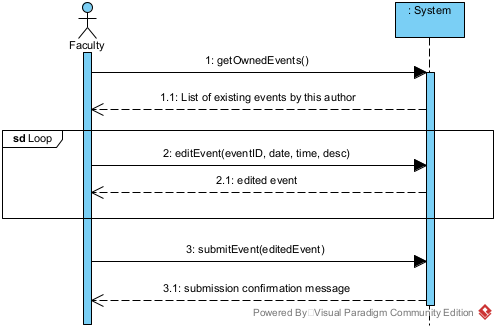
\includegraphics[scale=1.0]{images/SSD - UC05 - Edit Event.png}
    \caption{System sequence diagram for UC05: Edit Event}
    \label{fig:enter-label}
\end{figure}
\subsection{SSD for UC08: Submit Event for Review}
\begin{figure}[H]
    \centering
    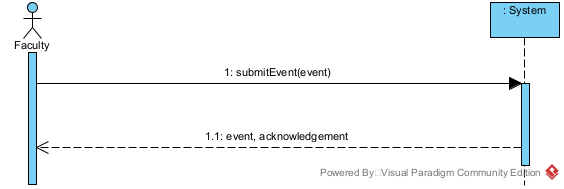
\includegraphics[scale=1.0]{images/SSD - UC08 - Submit for review.png}
    \caption{System sequence diagram for UC08: Submit Event for Review}
    \label{fig:enter-label}
\end{figure}
\subsection{SSD for UC11: Edit Post}
\begin{figure}[H]
    \centering
    \includegraphics[scale=1.0]{images/SSD - UC11 - Edit Post.png}
    \caption{System sequence diagram for UC11: Edit Posts}
    \label{fig:enter-label}
\end{figure}
\subsection{SSD for UC16: Manage media for display}
\begin{figure}[H]
    \centering
    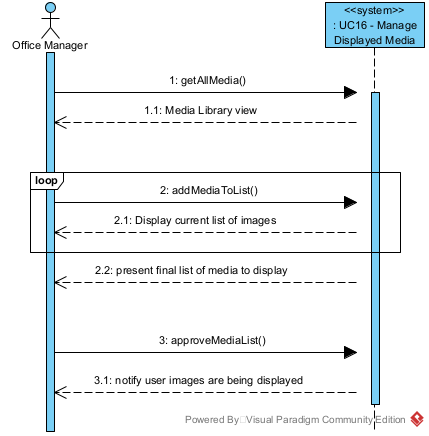
\includegraphics[scale=1.0]{images/SSD - UC16 - Manage Displayed Media.png}
    \caption{System sequence diagram for UC16: Manage media for display}
    \label{fig:enter-label}
\end{figure}
\section{System operations}
\begin{enumerate}
    \item scanQRCode()
    \item selectContentCategory(category)
    \item submitEvent(event)
    \item editPost(postId)
    \item updatePost(string)
    \item updatePost(media)
    \item submitForReview(post)
    \item getAllMedia()
    \item addMediaToList()
    \item approveMediaList()
    \item getOwnedEvents()
    \item editEvent(eventID, date, time, desc)
    \item submitEvent(editedEvent)
\end{enumerate}


\end{document}